\documentclass{ximera}

\newcommand{\RR}{\mathbb R}
\renewcommand{\d}{\,d}
\newcommand{\dd}[2][]{\frac{d #1}{d #2}}
\renewcommand{\l}{\ell}
\newcommand{\ddx}{\frac{d}{dx}}
\newcommand{\dfn}{\textbf}
\newcommand{\eval}[1]{\bigg[ #1 \bigg]}


\title[Dig-In:]{Polar coordinates}

\outcome{Work in polar coordinates.}
\outcome{Compute double integrals in polar coordinates.}

\begin{document}
\begin{abstract}
  We integrate over regions in polar coordinates.
\end{abstract}
\maketitle

We are currently interested in computing integrals of functions over
various regions in $\R^2$ and $\R^3$ via
\[
\underbrace{\iint_R F(x,y) \d A}_{\text{double integral}} \quad\text{and}\quad \underbrace{\iiint_R F(x,y,z) \d V}_{\text{triple integral}}
\]
Some regions like rectangles and boxes are easy to describe using
$(x,y)$-coordinates (a.k.a.\ rectangular coordinates). However, other
regions like circles and other things with \textit{rotational}
symmetry are easier to work with in polar coordinates. Recall that in
polar coordinates,
\begin{align*} 
  x(\theta) &= r(\theta) \cdot \cos(\theta)\\
  y(\theta) &= r(\theta) \cdot \sin(\theta)
\end{align*}
where $r(\theta)$ is a function of $\theta$.  When working with
parametric equations of this form, it is common to notate
\[
(r \cdot \cos(\theta), r\cdot \sin(\theta)) \quad\text{as}\quad (r,\theta)
\]
and state that we are working in \textit{polar coordinates}.

\begin{definition}
  An ordered pair consisting of a radius and an angle $(r,\theta)$
  can be graphed as
  \begin{align*}
    x &= r\cdot \cos(\theta)\\
    y &= r\cdot \sin(\theta)
  \end{align*}
  meaning:
  \begin{image}[2in]
    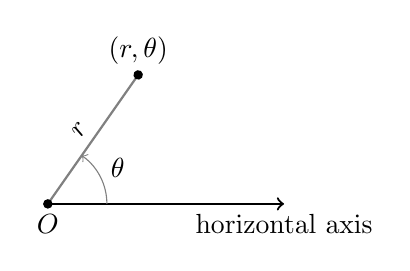
\begin{tikzpicture}
	\draw[thick,->] (0,0) node [below] {$O$} -- (3,0) node [below] {horizontal axis} ;
	\draw [thick,rotate=55,gray] (0,0)-- node [black,rotate=55,pos=.5,above] {$r$} (2,0) node [black,above] {$(r,\theta)$};
	\draw [->,gray] (.75,0) arc(0:55:.75); 
	\draw [rotate=27.5] (1,0) node {$\theta$};
        \filldraw (0,0) circle (1.5pt);
        \filldraw [rotate=55] (2,0) circle (1.5pt);
    \end{tikzpicture}
  \end{image}
  Coordinates of this type are called \dfn{polar coordinates}.
\end{definition}

\begin{question}
  Consider the point $(5, 2\pi/3)$ in polar coordinates. What is this
  point when expressed in $(x,y)$-coordinates?
  \begin{prompt}
    \[
    (x,y) = (\answer{5\cos(2\pi/3)}, \answer{5 \sin(2\pi/3)})
    \]
  \end{prompt}
  \begin{question}
    Consider the point $(-1, -5)$ in $(x,y)$-coordinates. What is this
    point when expressed in polar coordinates with $0\le\theta<2\pi$?
    \begin{prompt}
      \[
      (r,\theta) = (\answer{\sqrt{26}}, \answer{\arctan(5)+\pi})
      \]
    \end{prompt}
  \end{question}
\end{question}

\section{Double integrals in polar coordinates}

The basic form of the double integral is:
\begin{image}
  
\begin{tikzpicture}[scale=2,every node/.style={transform shape}]
    \node at (0,0) {
      $\color{green!70!black!70!blue}\iint_{\color{red!50!black}R} \color{purple!50!blue!90!black}F\color{blue!70!green} \d A$
    };
  \end{tikzpicture}
\end{image}
which can be interpreted as
\begin{quote}
  \textbf{Over \textcolor{red!50!black}{some region},
    \textcolor{green!70!black!70!blue}{sum up} products of
    \textcolor{purple!50!blue!90!black}{heights} and \textcolor{blue!70!green}{areas}.}
\end{quote}
Of course if you want to evaluate the integral (and honestly, who
doesn't?) you have to change $R$ to a region defined in $(x,y)$-coordinates,
and change $\d A$ to $\d x\d y$ or $\d y\d x$ leaving iterated integrals
\[
\int_a^b\int_c^d F(x,y) \d y \d x\quad\text{and}\quad \int_c^d \int_a^b F(x,y) \d x\d y
\]

Now consider representing a region $R$ with polar coordinates.
\begin{image}
  \begin{tikzpicture}
    \begin{axis}[
        tick label style={font=\scriptsize},axis y line=middle,axis x line=middle,name=myplot,%
	ymin=-.1,ymax=1.1,%
	xmin=-.2,xmax=1.24%
      ]
      \addplot [fill1,fill=fill1,area style] coordinates {(0.6928,0.4)(0.6857,0.412)(0.6784,0.4239)(0.6709,0.4357)(0.6632,0.4474)(0.6553,0.4589)(0.6472,0.4702)(0.6389,0.4815)(0.6304,0.4925)(0.6217,0.5035)(0.6128,0.5142)(0.6038,0.5248)(0.5945,0.5353)(0.5851,0.5456)(0.5755,0.5557)(0.5657,0.5657)(0.4243,0.4243)(0.4316,0.4168)(0.4388,0.4092)(0.4459,0.4015)(0.4528,0.3936)(0.4596,0.3857)(0.4663,0.3776)(0.4728,0.3694)(0.4792,0.3611)(0.4854,0.3527)(0.4915,0.3441)(0.4974,0.3355)(0.5032,0.3268)(0.5088,0.318)(0.5143,0.309)(0.5196,0.3)(0.6928,0.4)};

      \addplot [penColor,ultra thick, smooth,domain=0:90,samples=30] ({cos(x)*(1+.05*cos(9*x))},{sin(x)*(1+.05*cos(9*x))});

      \addplot [black, thick,smooth,domain=0:15,samples=30] ({cos(x)*(1.05)},{sin(x)*(1.05))});
      
      \addplot [black, thick,smooth,domain=15:30,samples=30] ({cos(x)*(.95)},{sin(x)*(.95))});
      %
      \addplot [black, thick,smooth,domain=30:45,samples=30] ({cos(x)*(1.05)},{sin(x)*(1.05))});
      %
      \addplot [black, thick,smooth,domain=45:60,samples=30] ({cos(x)*(.97)},{sin(x)*(.97))});
%
      \addplot [black, thick,smooth,domain=60:75,samples=30] ({cos(x)*(1)},{sin(x)*(1))});
      %
      \addplot [black, thick,smooth,domain=75:90,samples=30] ({cos(x)*(1.05)},{sin(x)*(1.05))});
      

      
      \addplot [black, thick,smooth,domain=0:90,samples=30] ({cos(x)*(.8)},{sin(x)*(.8))});
      
      \addplot [black, thick,smooth,domain=0:90,samples=30] ({cos(x)*(.6)},{sin(x)*(.6))});
      
      \addplot [black, thick,smooth,domain=0:90,samples=30] ({cos(x)*(.4)},{sin(x)*(.4))});

      \addplot [black, thick,smooth,domain=0:90,samples=30] ({cos(x)*(.2)},{sin(x)*(.2))});

      
      \addplot [black,thick, smooth,domain=0:1.05,samples=2] ({cos(15)*(x)},{sin(15)*(x)});

      \addplot [black,thick, smooth,domain=0:1.05,samples=2] ({cos(30)*(x)},{sin(30)*(x)});
      
      \addplot [black,thick, smooth,domain=0:1.05,samples=2] ({cos(45)*(x)},{sin(45)*(x)});

      \addplot [black,thick, smooth,domain=0:1,samples=2] ({cos(60)*(x)},{sin(60)*(x)});
      
      \addplot [black,thick, smooth,domain=0:1.05,samples=2] ({cos(75)*(x)},{sin(75)*(x)});
      
      \addplot [penColor,ultra thick, smooth,domain=0:90,samples=30] ({cos(x)*(1+.05*cos(9*x))},{sin(x)*(1+.05*cos(9*x))});
\end{axis}

\node [right] at (myplot.right of origin) {\scriptsize $0$};
\node [above] at (myplot.above origin) {\scriptsize $\pi/2$};
\end{tikzpicture}
\end{image}

Let $R$ be the region in the first quadrant bounded by the curve. We
can approximate this region using the natural shape of polar
coordinates: Portions of sectors of circles. In the figure, one such
region is shaded, shown below:

\begin{image}
  \begin{tikzpicture}
    \begin{axis}[
        width=2.5in,
        tick label style={font=\scriptsize},axis y line=none,axis x line=none,name=myplot,%
        %x=.37\marginparwidth,
        %y=.37\marginparwidth,
        %xtick={-1,1},
        %minor x tick num=1,% 
        %			extra x ticks={.33},
        %			extra x tick labels={$1/3$},
        %ytick={-1,1},
        %minor y tick num=1,%extra y ticks={-5,-3,...,7},%
        ymin=-.05,ymax=0.65,%
        xmin=-.1,xmax=.74%
      ]
      
      
      
      \addplot [fill1,fill=fill1,area style] coordinates
               {(0.6928,0.4)(0.6857,0.412)(0.6784,0.4239)(0.6709,0.4357)
                 (0.6632,0.4474)(0.6553,0.4589)(0.6472,0.4702)(0.6389,0.4815)
                 (0.6304,0.4925)(0.6217,0.5035)(0.6128,0.5142)(0.6038,0.5248)
                 (0.5945,0.5353)(0.5851,0.5456)(0.5755,0.5557)(0.5657,0.5657)
                 (0.4243,0.4243)(0.4316,0.4168)(0.4388,0.4092)(0.4459,0.4015)
                 (0.4528,0.3936)(0.4596,0.3857)(0.4663,0.3776)(0.4728,0.3694)
                 (0.4792,0.3611)(0.4854,0.3527)(0.4915,0.3441)(0.4974,0.3355)
                 (0.5032,0.3268)(0.5088,0.318)(0.5143,0.309)(0.5196,0.3)(0.6928,0.4)};
      
      \addplot [penColor, thick,smooth,domain=30:45,samples=30] ({cos(x)*(.8)},{sin(x)*(.8))});
      \addplot [penColor, thick,smooth,domain=30:45,samples=30] ({cos(x)*(.8)},{sin(x)*(.8))});
      \addplot [penColor, thick,smooth,domain=30:45,samples=30] ({cos(x)*(.6)},{sin(x)*(.6))});

      \addplot [gray,thick, ->,smooth,domain=0:.6,samples=2] ({cos(30)*(x)},{sin(30)*(x)});
      \addplot [gray,thick, smooth,domain=0:.6,samples=2] ({cos(45)*(x)},{sin(45)*(x)});

      \addplot [penColor,thick, smooth,domain=.6:.8,samples=2] ({cos(30)*(x)},{sin(30)*(x)});
      \addplot [penColor,thick, smooth,domain=.6:.8,samples=2] ({cos(45)*(x)},{sin(45)*(x)});

      \draw [rotate=30] (axis cs:.31,-.12) node [rotate=30] {$\underbrace{\rule{92pt}{0pt}}_{r}$};
      \draw [rotate=30] (axis cs:.71,-.12) node [rotate=30] {$\underbrace{\rule{30pt}{0pt}}_{\d r}$};
      %\draw [rotate=45] (axis cs:.41,-.03) node [rotate=45] {$\overbrace{\rule{120pt}{0pt}}^{r_2}$};
      \draw [thick,->,rotate=24,gray] (axis cs:.45,0) arc (0:13:80pt);
      \draw (axis cs: .4,.3) node {\scriptsize $\d \theta$};
      \draw (axis cs: .55,.4125) node {$\d A$};
    \end{axis}
  \end{tikzpicture}
\end{image}
From the picture above, we see that:
\begin{align*}
\d A &= \d r \cdot (r \d \theta) \\
&= r \d r \d \theta
\end{align*}
Moreover, recalling that the determinant of a $2\times 2$ matrix gives
the area of a parallelogram, we could also deduce the correct formula
for $\d A$ by setting
\begin{align*}
  x(r,\theta) = r \cos(\theta)\\
  y(r,\theta) = r \sin(\theta)
\end{align*}
and computing:
\begin{align*}
  \d A &= \left| \det
  \begin{bmatrix}
    \pp[x]{r} \d r & \pp[y]{r} \d r\\
    \pp[x]{\theta} \d \theta & \pp[y]{\theta} \d \theta
  \end{bmatrix}\right|\\
  &= \left| \det
  \begin{bmatrix}
    \answer[given]{\cos(\theta)} \d r & \answer[given]{\sin(\theta)} \d r\\
    \answer[given]{-r\sin(\theta)} \d \theta & \answer[given]{r\cos(\theta)} \d \theta
  \end{bmatrix}\right|\\
  &= r \d r \d \theta
\end{align*}


So to evaluate
\[
\iint_R F\d A,
\]
replace $\d A$ with $r\d r\d\theta$ and convert the function $z=F(x,y)$
to a function of polar coordinates:
\[
F(r\cos(\theta),r\sin(\theta))
\]
Finally, find bounds $g_1(\theta)\leq r\leq g_2(\theta)$ and
$\alpha\leq\theta\leq\beta$ that describe $R$. Let's state this as a
theorem:

\begin{theorem}[Fubini]
  Let $F:\R^2\to\R$ be continuous on the region
  \[
  R=\{(r,\theta):\text{$\alpha\leq\theta\leq\beta$ and $g_1(\theta)\leq r\leq g_2(\theta)$}\}
  \]
  Then: 
  \[
  \iint_R F(x,y)\d A = \int_\alpha^\beta\int_{g_1(\theta)}^{g_2(\theta)} F\big(r\cos(\theta),r\sin(\theta)\big) r\d r\d \theta.
  \]
\end{theorem}

\begin{question}
  Write down a double integral in polar coordinates that will compute
  the area of a circle of radius $a$.
  \begin{prompt}
  \[
  \iint_R \d A = \int_{\answer{0}}^{\answer{2\pi}}
  \int_{\answer{0}}^{\answer{a}}r \d r \d \theta 
  \]
  \end{prompt}
\end{question}

%%
%% This problem is messed up, and I cannot fix it.
%%
%% \begin{question}
%%   Below we give the values of a function $F:\R^2\to \R$ on a polar
%%   region. 
%%   \begin{image}
%%     \begin{tikzpicture}
%%       \begin{polaraxis}[width=5in,
%%           domain=0:360,
%%           xtick={0,45,...,360},
%%           xticklabels={$0$,$\frac{\pi}{4}$,$\frac{\pi}{2}$,$\frac{3\pi}{4}$,$\pi$,$\frac{5\pi}{4}$,$\frac{3\pi}{2}$,$\frac{7\pi}{4}$,$2\pi$},
%%           ytick={.5,1},
%%         ]
%%         \addplot[fill=none,draw=none,domain=-60:60]{1};
%%         \node[penColor] at (axis cs: 22.5,.3) {\Huge$4$};
%%         \node[penColor] at (axis cs: 22.5,.75) {\Huge$2$};

%%         \node[penColor] at (axis cs: 67.5,.3) {\Huge$5$};
%%         \node[penColor] at (axis cs: 67.5,.75) {\Huge$1$};

%%         \node[penColor] at (axis cs: 112.5,.3) {\Huge$5$};
%%         \node[penColor] at (axis cs: 112.5,.75) {\Huge$0$};

%%         \node[penColor] at (axis cs: 157.5,.3) {\Huge$4$};
%%         \node[penColor] at (axis cs: 157.5,.75) {\Huge$-1$};

%%         \node[penColor] at (axis cs: 202.5,.3) {\Huge$2$};
%%         \node[penColor] at (axis cs: 202.5,.75) {\Huge$-3$};

%%         \node[penColor] at (axis cs: 247.5,.3) {\Huge$3$};
%%         \node[penColor] at (axis cs: 247.5,.75) {\Huge$0$};

%%         \node[penColor] at (axis cs: 292.5,.3) {\Huge$3$};
%%         \node[penColor] at (axis cs: 292.5,.75) {\Huge$1$};

%%         \node[penColor] at (axis cs: 337.5,.3) {\Huge$4$};
%%         \node[penColor] at (axis cs: 337.5,.75) {\Huge$1$};
%%       \end{polaraxis}
%%     \end{tikzpicture}
%%   \end{image}
%%   Let $F(r,\theta)$ be determined by the ``outer-value'' of $r$ and
%%   the ``smaller-angle'' of $\theta$ for the region containing the value
%%   for $F$. For example: $F(0.5,\pi/4) = 4$ and $F(1,\pi/4) = 2$.  Let
%%   \[
%%   R = \{(r,\theta): \text{$\pi/4 \le \theta \le 5\pi/4$ and $0\le r\le 1$}\}
%%   \]
%%   Using the table above, estimate:
%%   \[
%%   \iint_R F(r,\theta) \d A
%%   \begin{prompt}
%%     = \answer{5\pi/8}
%%   \end{prompt}
%%   \]
%%   \begin{hint}
%%     Remember,
%%     \[
%%     \iint_R F(r,\theta)\d A = \int_{\pi/4}^{5\pi/4}\int_{0}^1 F(r,\theta) r\d r\d \theta.
%%     \]
%%   \end{hint}
%% \end{question}

\begin{example}
  Compute the area of the
  \link[lemniscate]{http://en.wikipedia.org/wiki/Lemniscate} given by:
  \[
  r(\theta) = \sqrt{\cos(2\theta)}
  \]
  \begin{explanation}
    When first exploring problems like this, we should try to plot them if we can.
    \begin{onlineOnly}
      \[
      \graph[polar,xmin=-2, xmax=2, ymin=-1.5, ymax=1.5]{r=\sqrt{\cos(2\theta)}}
      \]
    \end{onlineOnly}
    Now either by reasoning about cosine, or by experimenting with the
    plot, we should convince ourselves that if $0\le \theta\le \pi/4$,
    the area is given by:
    \begin{align*}
      4\int_{0}^{\pi/4} \int_{0}^{\sqrt{\cos(2\theta)}}\answer[given]{r} \d r \d \theta
      &= 4\int_{0}^{\pi/4} \eval{\answer[given]{r^2/2}}_{\answer[given]{0}}^{\answer[given]{\sqrt{\cos(2\theta)}}}  \d \theta\\
      &= 4\int_{0}^{\pi/4} \answer[given]{\cos(2\theta)/2}  \d \theta\\
      &= \int_{0}^{\pi/4} \answer[given]{2\cos(2\theta)}  \d \theta\\
      &= \eval{\answer[given]{\sin(2\theta)}}_{\answer[given]{0}}^{\answer[given]{\pi/4}}  \\
      &= \answer[given]{1}
    \end{align*}
  \end{explanation}
\end{example}

Finally, let's derive the volume of a sphere using a double integral
in polar coordinates.

\begin{example}
  Find the volume of a sphere with radius $a$.
  \begin{explanation}
    The sphere of radius $a$, centered at the origin, has equation
    \[
    \answer[given]{x^2+y^2+z^2}=a^2
    \]
    Solving for $z$, we have
    $z=\answer[given]{\sqrt{a^2-x^2-y^2}}$. This gives the upper half
    of a sphere. We wish to find the volume under this top half, then
    double it to find the total volume.

    The region we need to integrate over is the circle of radius $a$,
    centered at the origin.
    \[
    R =\{(r,\theta):\text{$\answer[given]{0}\leq r\leq \answer[given]{a}$ and  $\answer[given]{0}\leq\theta\leq\answer[given]{2\pi}$}\}
    \]
    Thus, the volume of a sphere with radius $a$ is:
    \[
    2\iint_R\sqrt{a^2-x^2-y^2}\d A
    \]
    \begin{align*}
      &= 2\int_{\answer[given]{0}}^{\answer[given]{2\pi}}\int_{\answer[given]{0}}^{\answer[given]{a}}\sqrt{a^2-(r\cos\theta)^2-(r\sin\theta)^2}r\d r\d\theta\\
      &=2\int_{\answer[given]{0}}^{\answer[given]{2\pi}}\int_{\answer[given]{0}}^{\answer[given]{a}}r\sqrt{a^2-r^2}\d r\d\theta\\
      &=2\int_{\answer[given]{0}}^{\answer[given]{2\pi}}\eval{\answer[given]{\frac{-2}{6}(a^2-r^2)^{3/2}}}_{0}^a \d\theta\\
      &= \int_{\answer[given]{0}}^{\answer[given]{2\pi}}\left(\answer[given]{\frac{2}{3}a^3}\right)\d \theta\\
      &=\eval{\answer[given]{\frac{2}{3}a^3\theta}}_{\answer[given]{0}}^{\answer[given]{2\pi}}\\
      &=\answer[given]{\frac{4}{3}\pi a^3}.
    \end{align*}
    The formula for the volume of a sphere with radius $r$ is given as
    $4/3\pi r^3$.  We have justified this formula with our
    calculation!
  \end{explanation}
\end{example}

One may wonder how polar coordinates could be extended to triple integrals\dots read on!


\end{document}
